%% This is an example first chapter.  You should put chapter/appendix that you
%% write into a separate file, and add a line \include{yourfilename} to
%% main.tex, where `yourfilename.tex' is the name of the chapter/appendix file.
%% You can process specific files by typing their names in at the 
%% \files=
%% prompt when you run the file main.tex through LaTeX.
%% prompt when you run the file main.tex through LaTeX.
\chapter{Use of a Global Model to Understand Atmospheric Mercury Observations at Monitoring Sites in Latin America }\label{chapter2}
%% BACKGROUND
\begin{flushleft}
Environmental pollution from Hg damages ecosystems through Hg's transformation into toxic methylmercury and bio-accumulation in food chains. Further, Hg is highly mobile in the atmosphere, allowing it to travel to faraway places, resulting in worldwide distribution of its elemental form, \hg, which can last for as long as six months in the atmosphere\cite{horowitz_new_2017,shah_improved_2021}. Hg in the atmosphere can be classified as gaseous elemental Hg (GEM), gaseous oxidized Hg (GOM), and particulate-bound Hg (PBM)  \cite{lindberg_synthesis_2007,schroeder_atmospheric_1998,landis_development_2002}. In most cases, Hg emissions occur as gaseous elemental \hg, which is relatively inert and sparingly soluble in water \cite{horowitz_new_2017}. Since most Hg entering ecosystems comes from the atmosphere, monitoring and modeling atmospheric Hg and Hg deposition enables us to understand its biogeochemical cycle. In addition, a better understanding of Hg's circulation in the environment would enable effective policies to reduce its harmful effects.
\end{flushleft}
\begin{flushleft}
 In this chapter, we compare the outputs of the GEOS-Chem model with observed Hg at multiple sites in Latin America from two monitoring networks. We combine simulations of Hg in the atmosphere produced by the \gc CTM (Sect. \ref{c2_geos_chem_simulations} - Sect. \ref{c2_geos_chem_simulations}) with ground-based observations of atmospheric total gaseous mercury (TGM) (Sect. \ref{c2_monitoring_site_characteristics}) from the Global Mercury Observation System (GMOS)\cite{sprovieri_atmospheric_2016} and gaseous elemental mercury (GEM) data from a network of passive air samplers (PAS)\cite{quant_measuring_2021} distributed across Latin America. Then, we present comparisons between observations and model outputs and discuss the implications of the current state of atmospheric monitoring and modeling atmospheric Hg in Latin America(Sect. \ref{c2_results}). Finally, we summarize conclusions from the analysis (Sect. \ref{c2_conclusion}).
\end{flushleft}
\section{Background}\label{chapter2_background}
\begin{flushleft}

Hg monitoring networks and atmospheric Hg models are closely interconnected in the literature. For instance, Gustin et al's.\cite{gustin_mercury_2020} describe up-to-date scientific thinking regarding mercury in the environment, monitoring and modeling techniques, and how they relate to Minamata Convention on Mercury.  Notably, the mutual dependency between atmospheric modeling and monitoring is presented in the MC's "Monitoring Guidance Document"\cite{unep_guidance_2021}, which states that observations are needed not only to detect and quantify changes but also to improve and evaluate models of mercury transport, fate, exposure, and impacts\cite{unep_guidance_2021}. Similarly, Sprovieri et al.\cite{sprovieri_atmospheric_2016} emphasize the importance of consistent global Hg measurements to validate regional and global-scale models.  According to Brasseur and Jacob\cite{brasseur_modeling_2017}, it is crucial to have a large ensemble of observations to evaluate atmospheric modeling outputs.

\end{flushleft}
Data from passive and active sampling sites are evaluated in this thesis. The MC's "Monitoring Guidance Document"\cite{unep_guidance_2021} provides a comprehensive definition and comparison of active and passive air sampling. Active air samplers, particularly automated ones, can deliver high-frequency data in a short period from as little as 5 seconds to 5 minutes\cite{unep_guidance_2021}. However, they may be complex and costly to set up and operate. In contrast to active samplers, PAS are low-cost, inexpensive, and do not require electricity, moving parts, pump operation, or calibration\cite{macagnano_passive_2018}. Despite their small size, they can be deployed at background, remote, urban, and hotspot sites without worrying about media failures\cite{unep_guidance_2021}. 
\begin{flushleft}
\end{flushleft}

\begin{flushleft}
Some world regions, such as Latin America and Africa, with high ASGM Hg emissions, have not been subject to detailed model-observation comparisons. This may be attributed to these regions' lack of wide coverage of required high-frequency atmospheric Hg monitoring capacity, as shown in Figure \ref{fig:global-hg-monitoring-networks}, which illustrates the distribution of different Hg monitoring networks worldwide\cite{united_nations_environment_programme_technical_2019}. It is evident in Figure \ref{fig:global-hg-monitoring-networks} that Latin America, Africa, and South East Asia remain significantly behind Europe and North America regarding access to large observation ensembles. A majority of the sampling sites present in these regions are PASs. 
\end{flushleft}

\begin{figure}[H]
  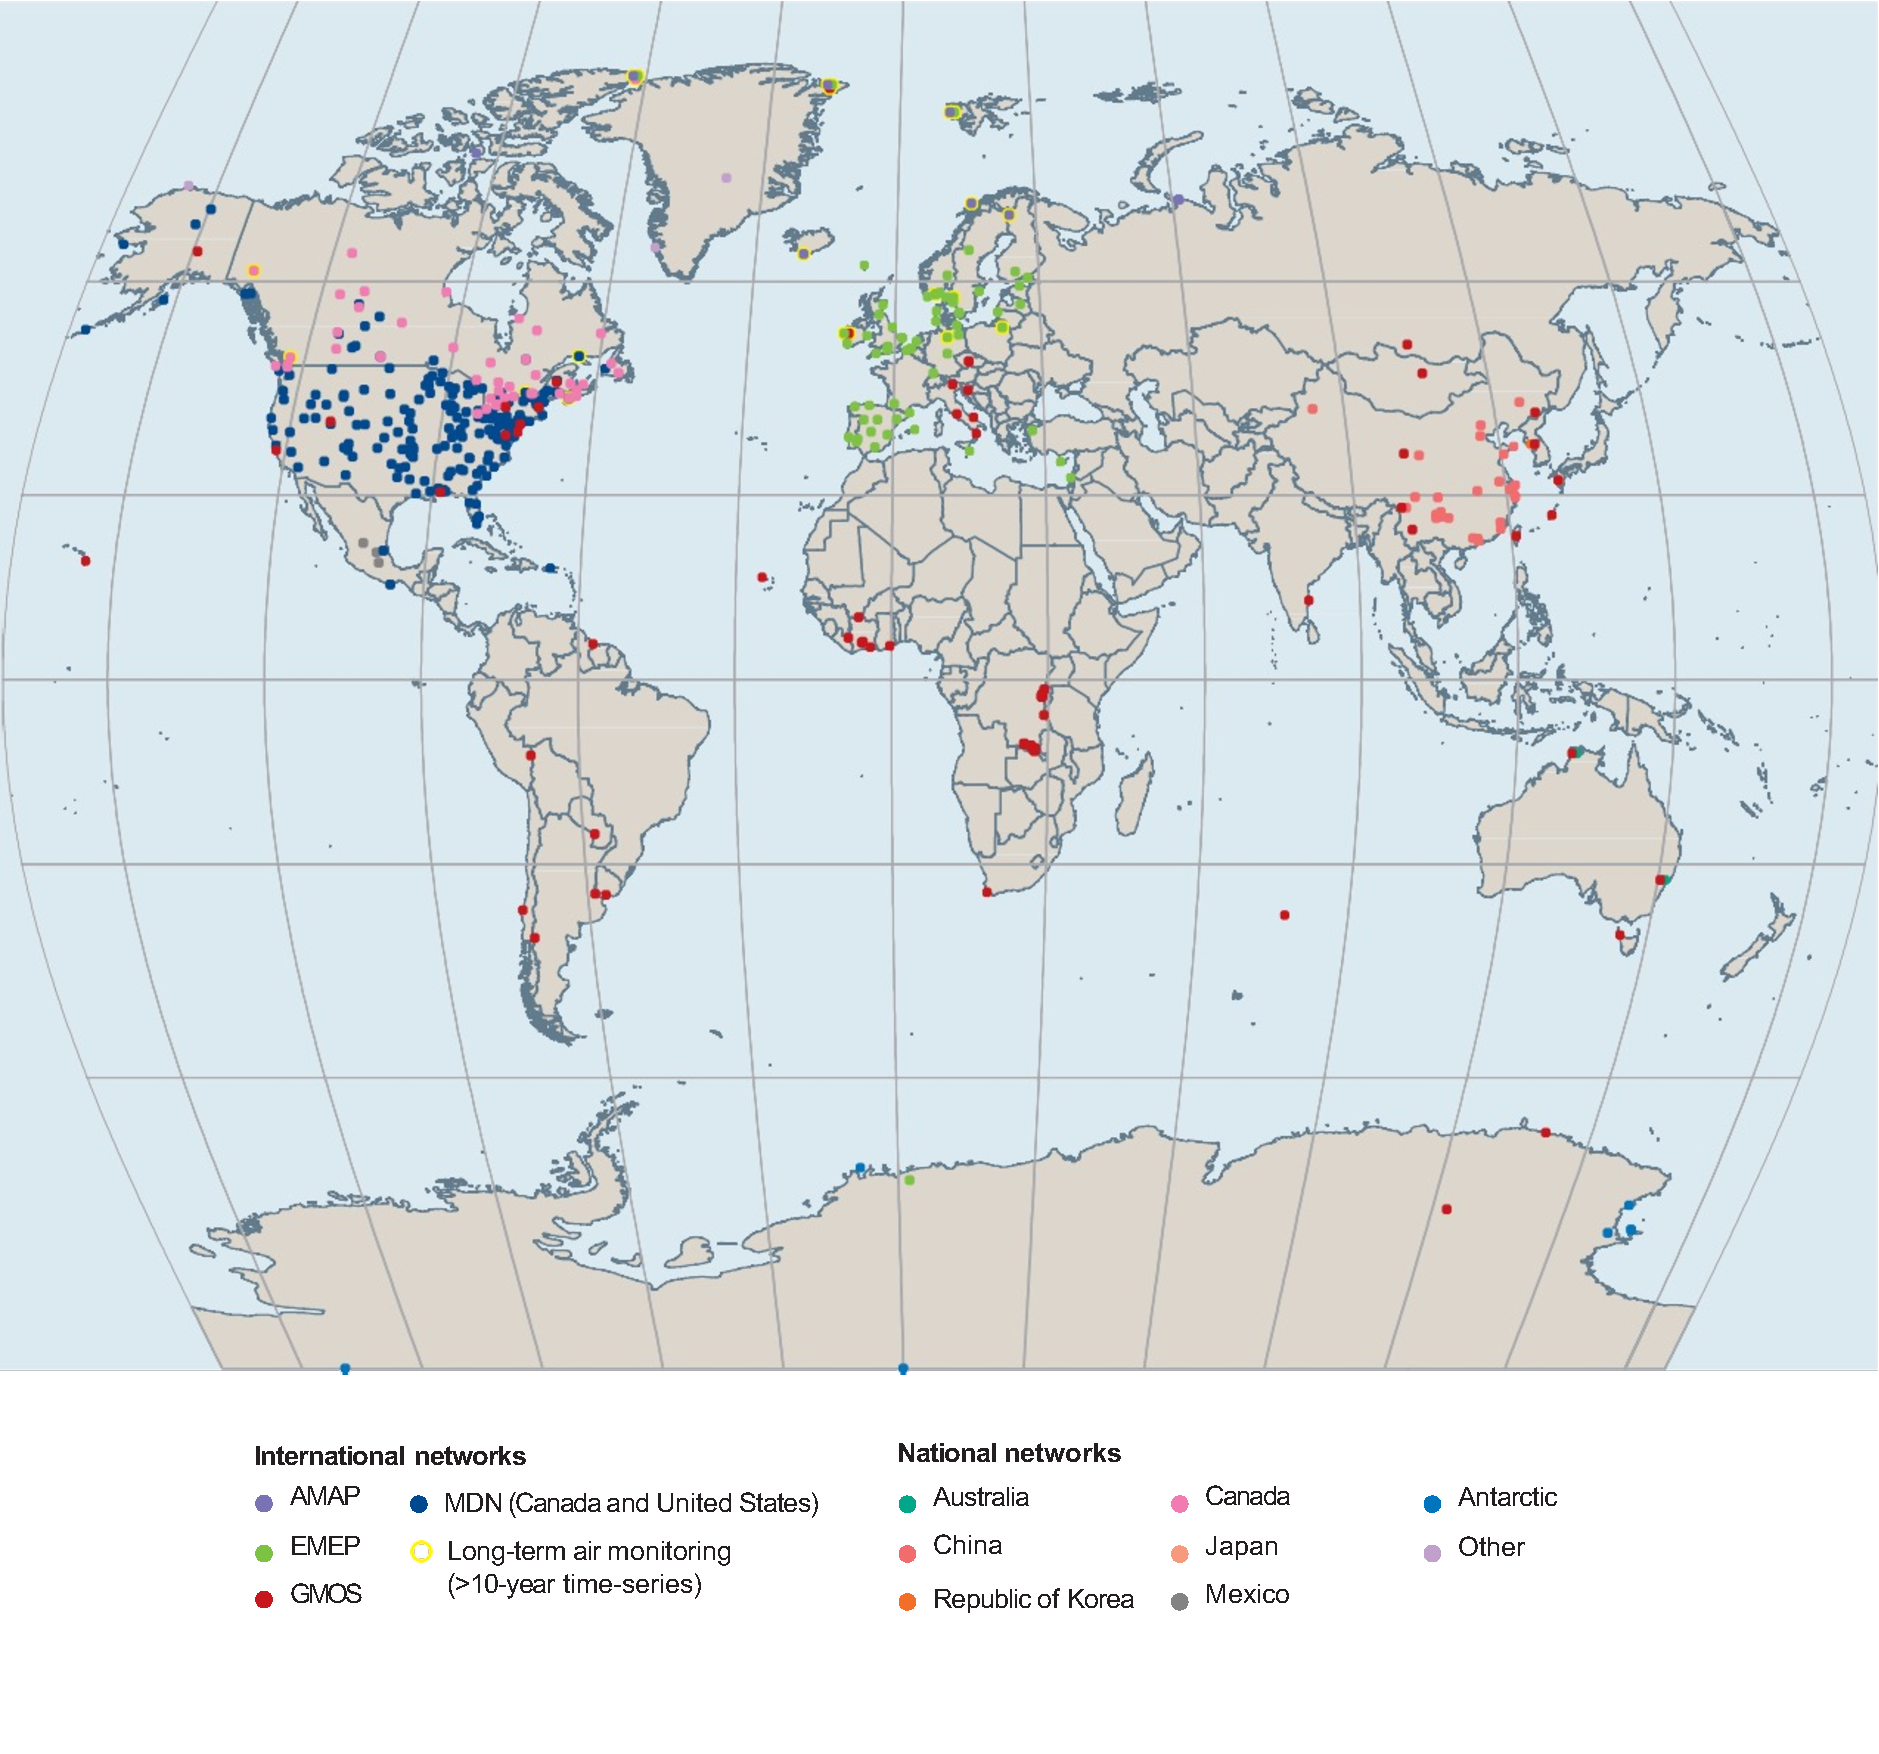
\includegraphics[width=\textwidth]{templates/figures/global-hg-monitoring-networks.pdf}
  \caption[Global map of Hg monitoring networks]{Global map of Hg monitoring networks \cite{united_nations_environment_programme_technical_2019}}
  \label{fig:global-hg-monitoring-networks}
  \centering
  
\end{figure}
\FloatBarrier






%%----------------------------METHODS-------------------------------------------
\section{Methods}\label{c2_methods}
\subsection{GEOS-Chem Description}\label{c2_geos_chem_description}
\begin{flushleft}

The global atmospheric Hg concentration was simulated using version 12.8.1 of GEOS-Chem, whose Hg simulation is described by Horowitz et al.\cite{horowitz_new_2017}. All the simulations in this study were run globally for 47 vertical layers at a resolution of 2.0$\times$2.5, which is approximately equal to a 222 km$\times$277.5 km grid square at the equator \cite{horowitz_new_2017}. Moreover, the MERRA-2 assimilated meteorological data \cite{gelaro_modern-era_2017} drive the model's atmospheric transport, which calculates atmospheric Hg from three tracers: elemental Hg, Hg\textsuperscript{0}, divalent Hg, Hg\textsuperscript{2+}, and particulate-bound divalent Hg, Hg\textsuperscript{p}. The Hg chemical scheme in the GEOS-Chem version used in this study considers bromine (Br) to be the primary \hg oxidant\cite{horowitz_new_2017} and employs monthly mean Br oxidant concentrations from Schmidt et al.\cite{schmidt_modeling_2016}. 
\end{flushleft}

\begin{flushleft}

\subsection{GEOS-Chem Simulations}\label{c2_geos_chem_simulations}

The GMA 2018 emissions inventory was used to represent anthropogenic emissions sources from all sectors\cite{steenhuisen_development_2019}. Different inputs to the GEOS-Chem model, such as emissions sources, can be toggled on or off depending on the research objective; hence a reference simulation, \on was created by turning on all Hg emissions sources globally. Moreover, a \off was generated by turning off the ASGM source globally to evaluate the contribution of ASGM to the baseline modeled Hg$^0$ in the atmosphere by calculating the difference between the \on and \off. Table \ref{tab:geos_chem_simulation_description} describes the simulations that were conducted in detail.
\end{flushleft}

\begin{table}[H]
\captionof{table}{GEOS-Chem simulations conducted}
\label{tab:geos_chem_simulation_description}

\centering
\resizebox{\textwidth}{!}{\begin{tabular}{lccp{0.6\linewidth}}

\hline
Simulation Name &Period & Resolution & Description  \\
                        
\hline
Base (ASGM=ON)      & 2010-2016     & 2.0$\times$2.5 & All Hg anthropogenic emission sources are turned on  \\
No ASGM (ASGM=OFF)  & 2010-2016     & 2.0$\times$2.5 & All ASGM emissions are turned off\\
\hline
\end{tabular}}
\end{table}

\begin{flushleft}
 The simulation frequency was set to output daily \hg averages at the global scale, while the \hg output for the grid boxes corresponding to the locations of the GMOS observation sites was set to an hourly frequency. The GEOS-Chem outputs for all the simulations were in units of parts per trillion (ppt) and were converted to \nang at standard temperature and pressure (273 K, 1 atm) to compare them to observations.
\end{flushleft}

\subsection{Atmospheric Mercury Monitoring Sites in Latin America} \label{c2_monitoring_site_characteristics}
\begin{flushleft}
 The GMOS network is one of a few major projects to develop a global observing system for Hg pollution. GMOS aims to provide high-quality Hg data sets in the Northern and Southern hemispheres to enable a more comprehensive assessment of atmospheric Hg concentrations and their dependence on meteorology, long-range atmospheric transport, and atmospheric emissions\cite{sprovieri_atmospheric_2016}. A vast network of ground-based monitoring stations, regular oceanographic cruises, and lower, upper, and stratospheric measurements make up this European Union-funded project \cite{koenig_seasonal_2021,sprovieri_atmospheric_2016}. More than 40 ground-based monitoring sites constitute the GMOS network, covering many regions with limited to no observational data before GMOS\cite{sprovieri_atmospheric_2016}. The GMOS monitoring network has five sites in Latin America that actively monitor Hg levels. A detailed analysis of the Sisal, Calhau, Manaus, Nieuw Nickerie, and Bariloche sites was conducted by Sprovieri et al.\cite{sprovieri_atmospheric_2016}, and the Chalcataya site was analyzed in detail by Koenig et al.\cite{koenig_seasonal_2021}. A summary of the sites' characteristics is shown in Table \ref{tab:gmos_sites_info}. Moreover, the distribution of these GMOS sites in Latin America is indicated by the red triangles in Figure \ref{fig:Latam_Passive_SamplerSites}, which is a map showing the names and locations of the GMOS Monitoring Network Sites and Passive Sampler sites in Latin America \cite{quant_measuring_2021,koenig_seasonal_2021}. Moreover, PAS data from the Latin American Passive Air sampling Network (LAPAN), which was analyzed in detail by Quant et al.\cite{quant_measuring_2021}, was used for the model observation comparison. The respective locations of the PAS sites are shown by the blue circles in Figure \ref{fig:Latam_Passive_SamplerSites}.
 %A primary objective of this study was to evaluate the degree to which ASGM Hg emissions affected the Hg concentrations in the atmosphere at regional and global scales, so high-frequency GMOS data were collected to facilitate this evaluation.
  \end{flushleft}
  
  \begin{table}[H]
\captionof{table}[Characteristics of the GMOS sites evaluated]{Characteristics of the GMOS sites evaluated \cite{koenig_seasonal_2021,sprovieri_atmospheric_2016}. }
\label{tab:gmos_sites_info}

\centering
\resizebox{\textwidth}{!}{\begin{tabular}{llccp{0.2\linewidth}rcll}
  \hline

Site                        & Site      & Latitude  & Longitude & Physical  & Elevation    & Number of      & Site &  Measurement  \\
                            & abbrev    &           &           &  Setting  & (m)           & Records (days) & Type&   Period \\
\hline
Sisal, Mexico               & SIS       & 21.16     & -90.05    &   Coastal site        &   7           &   320 &   Secondary    & 1/1/2010-1/1/2016   \\
Calhau, Cape Verde          & CAL       & 16.86     & -24.87    &   Coastal site        &   10          &   309 &   Secondary   & 1/1/2013-12/1/2014  \\
Nieuw Nickerie, Suriname    & NIK       & 5.93      & -56.98    &   Coastal site        &   1           &   215 &    Secondary   & 3/1/2007-12/1/2014 \\
Manaus, Brazil              & MAN       & -2.89     & -59.96    &    Amazon site       &  110          &   100 &   Master   & 1/1/2013-12/1/2014 \\
Chalcataya, Bolivia         & CHC       & -16.2     & -68.12    &    Mountain site       &  5340         &   333 &    Secondary   & 7/1/2014-2/1/2016  \\
Bariloche, Agentina         & BAR       & -41.13    & -72.42    &    Mountain site       &  800          &   333 &  Master     & 10/1/2012-7/1/2017 \\
  \hline
\end{tabular}}

\end{table}

  
 \begin{flushleft}
  The GMOS sites are classified as either secondary or master sites in Table\ref{tab:gmos_sites_info} to indicate the type of data collected and the type of equipment used at the site. Master stations are those where Gaseous Elemental Hg (GEM, i.e., the gas phase Hg in its ground electronic state), Gaseous Oxidized Hg (GOM, i.e., the oxidized gas phase Hg compounds), Hg associated with suspended particulate matter (PBM2.5) and Hg in precipitation are continuously measured while secondary stations are those where only GEM and Hg in precipitation are continuously measured \cite{sprovieri_atmospheric_2016,gustin_measuring_2015,koenig_seasonal_2021}.
\end{flushleft}


\begin{figure}[H]
 \centering
  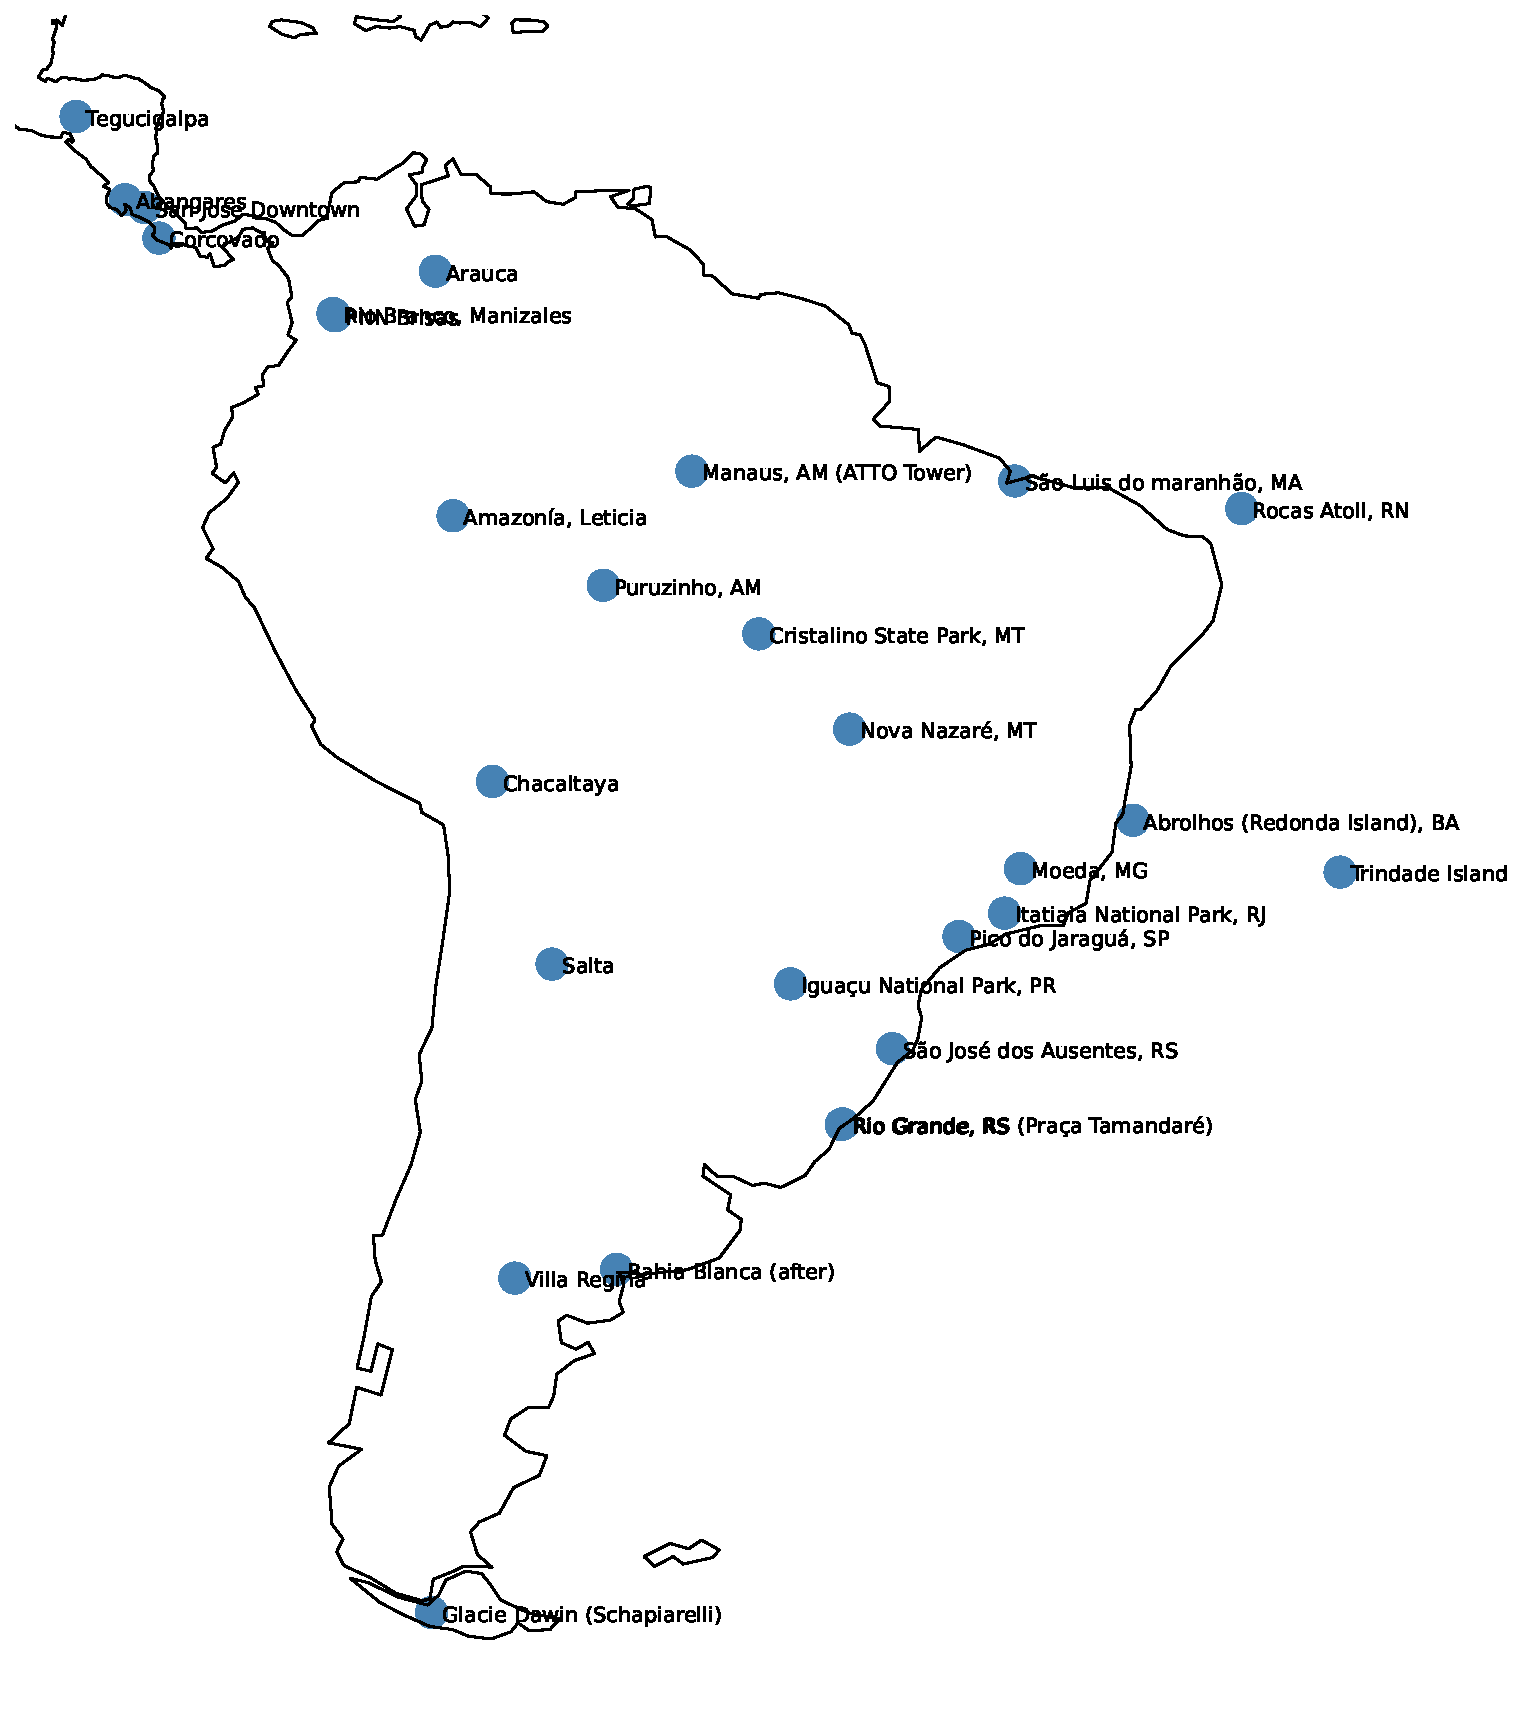
\includegraphics[width=0.8\textwidth]{templates/figures/Passive_Samplers/Latam_Passive_SamplerSites.pdf}
  \caption[Map showing the names and locations of the GMOS Monitoring Network Sites and Passive Sampler sites in Latin America.]{Map showing the names and locations of the GMOS Monitoring Network Sites and Passive Sampler sites in Latin America. GMOS sites are indicated by the red triangles, and the PAS sites are indicated by the blue dots\cite{quant_measuring_2021,koenig_seasonal_2021}.}
  \label{fig:Latam_Passive_SamplerSites}
\end{figure}
\FloatBarrier

\subsection{Pre-processing and Comparison of Observed and Modeled Mercury Concentration in the Atmosphere}\label{c2_observation_data_manipulation}
\begin{flushleft}
  Annual average GEM concentration data for 27 PAS sites in Latin America was obtained from Quant et al.\cite{quant_measuring_2021}, which included information about the coordinates of the deployment sites and the period of measurement. The PAS data was already \nang hence there was no need for pre-processing before comparison with the modeled Hg concentrations. Furthermore, the PAS had been deployed for a year; the different deployment dates ranged from October 20th, 2017, to March 14th, 2020. Therefore the annual average GEM concentrations from the PASs were compared to the modeled annual average \hg for 2015 for each site. 
  \end{flushleft}

\begin{flushleft}
  Available Hg observation data from the GMOS stations on Figure  \ref{fig:Latam_Passive_SamplerSites} was obtained from the GMOS online database (http://www.gmos.eu), as well as published studies about the Hg monitoring data from the different sites  \cite{sprovieri_atmospheric_2016,koenig_seasonal_2021}. The data sets were pre-processed based on the information in Sprovieri et al.\cite{sprovieri_atmospheric_2016} and Koenig et al.\cite{koenig_seasonal_2021}. Daily and annual averages of the observed TGM concentration were calculated to compare with the \gc output. 
\end{flushleft}





%%----------------------------RESULTS AND DISCUSSION---------------------------
\section{Results and Discussion}\label{c2_results}
\begin{figure}[H]
\centering
  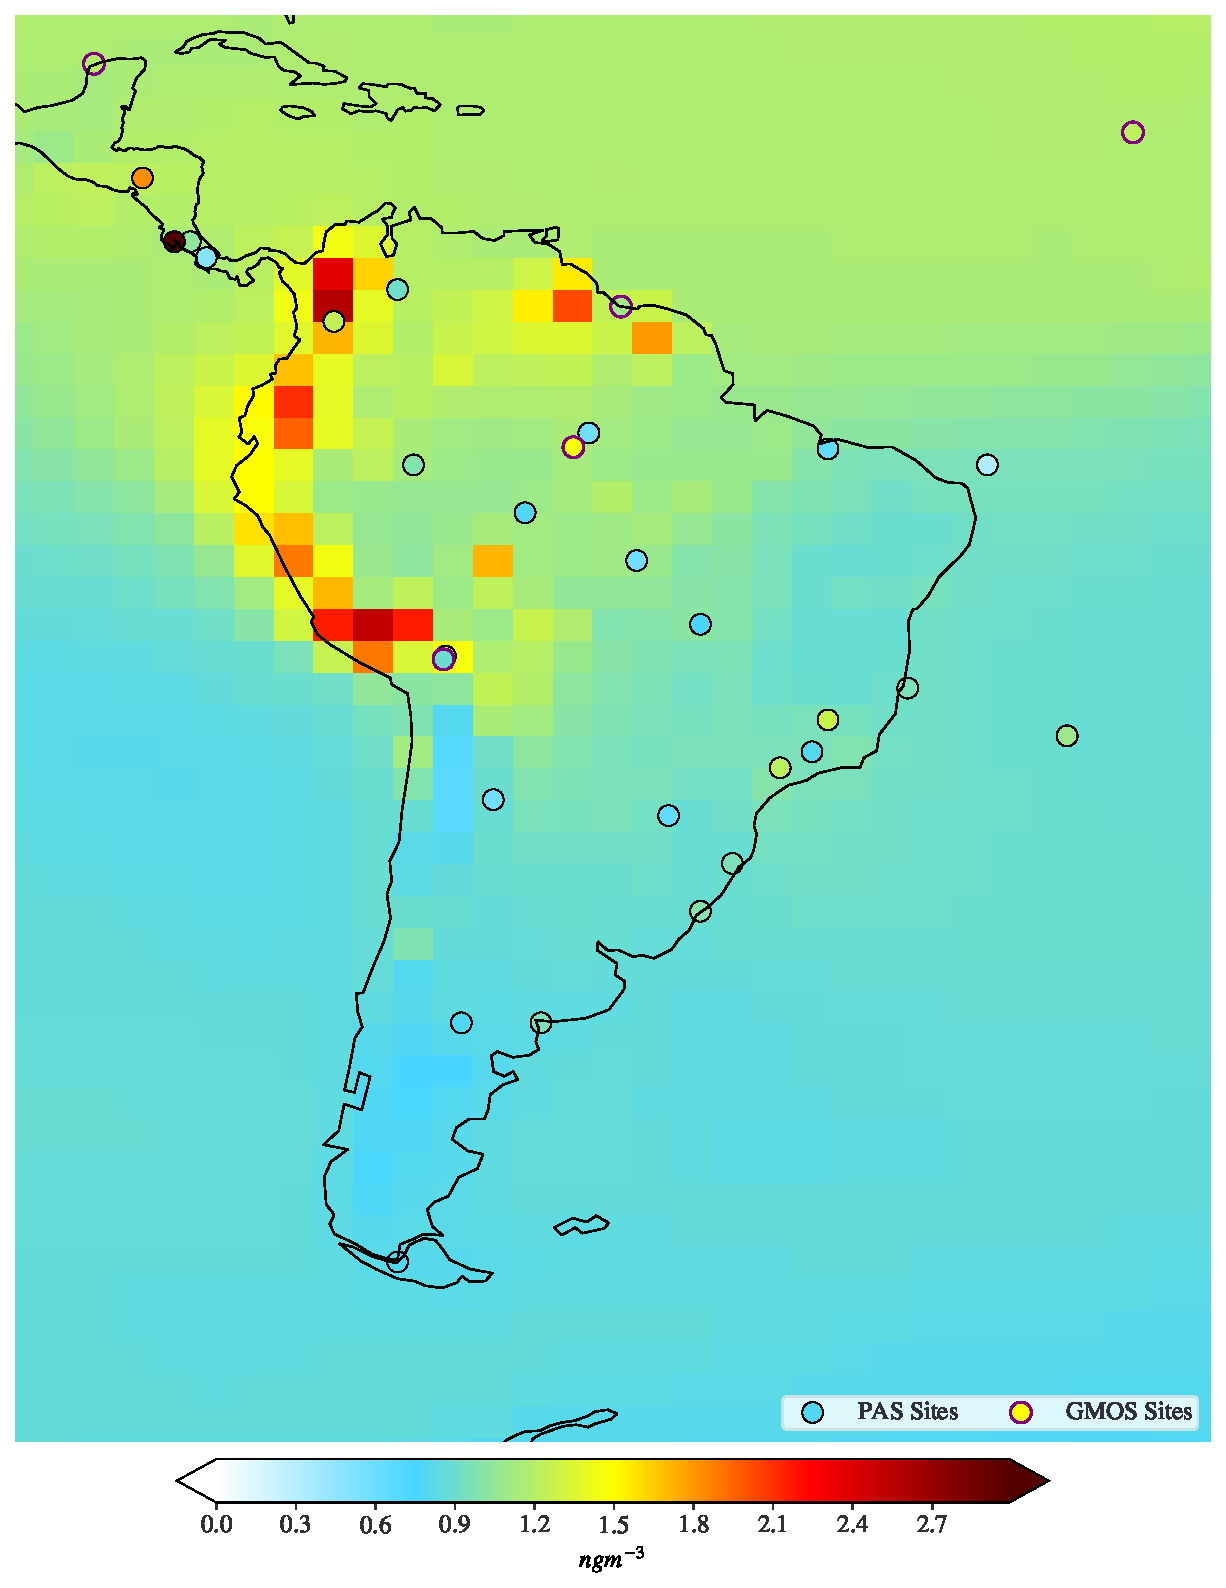
\includegraphics[width=0.75\textwidth]{templates/figures/Passive_Samplers/07-27-22_pas_vs_model_Hg0-per-year_001.pdf}
  \caption[The average annual Hg concentration on Latin America's surface. ]{The average annual Hg concentration on Latin America's surface. The background is the yearly average \hg concentration generated by the Base (ASGM=ON) simulation for 2015. Circles represent the annual average GEM concentration at PAS sites, while triangles represent the yearly average TGM concentration at GMOS sites\cite{sprovieri_atmospheric_2016,quant_measuring_2021,koenig_seasonal_2021}.}
  \label{fig:06-12-22_pas_vs_model_Hg0-per-year_001}
  
  
\end{figure}
\FloatBarrier
\begin{flushleft}
 Recent publications analyzing global Hg monitoring data highlight an observed inter-hemispheric gradient of Hg concentration where Hg concentration in the southern hemisphere is lower than Hg concentration in the northern hemisphere\cite{united_nations_environment_programme_technical_2019,sprovieri_atmospheric_2016}. The gradient is evident in the simulated background annual average \hg concentration as seen in Figure \ref{fig:06-12-22_pas_vs_model_Hg0-per-year_001}. Moreover, most GMOS sites agree with and validate the modeled interhemispheric gradient. However, a glance at Table \ref{tab:model_percentage_overestimation_of_mean} shows that the model overestimates the annual average Hg concentration at all the GMOS sites. Moreover, Figure \ref{fig:gmos_sites_stats} better visualizes the difference between the modeled and observed concentrations. The bar chart in Figure \ref{fig:gmos_sites_stats} compares observed and modeled Hg concentrations at the GMOS sites. Observed concentrations are indicated in red, modeled in blue, and ASGM contribution in green. There are annotations on the bars indicating the average concentration of Hg. In addition, each bar is annotated above with the data set's standard deviation and error bars.
\end{flushleft}



\begin{table}[H]
\captionof{table}[Comparison of the modeled \hgc and the observed TGM concentrations at the GMOS sites.]{Comparison of the modeled \hgc and the observed TGM concentrations at the GMOS sites. The percentage difference between the model predictions and the observations depicts the extent to which the model predicts the observed TGM concentrations }
\label{tab:model_percentage_overestimation_of_mean}

\center
\resizebox{\textwidth}{!}{\begin{tabular}{lcccc}
  \hline
GMOS Site   & Observed Average TGM/GEM  & Modeled Average \hg   &  Percentage difference between    &   Percentage ASGM\\
            &  Concentration (\nang )   & Concentration (\nang) &  modeled and observed average (\%)    &   Contribution (\%) \\
                        
\hline
Sisal          &     1.15               &             1.26               & 10                                   & 9 \\
Calhau         &     1.22               &             1.29               & 6                                    & 9 \\
Nieuw Nickerie &     1.17               &             1.41               & 20                                   & 16\\
Manaus         &     1.01               &             1.26               & 25                                   & 18 \\
Chalcataya     &     1.04               &             1.21               & 17                                   & 23 \\
Bariloche      &     0.71               &             0.9                & 27                                   & 6 \\
  \hline
\end{tabular}}
\end{table}
\FloatBarrier
\begin{figure}[H]
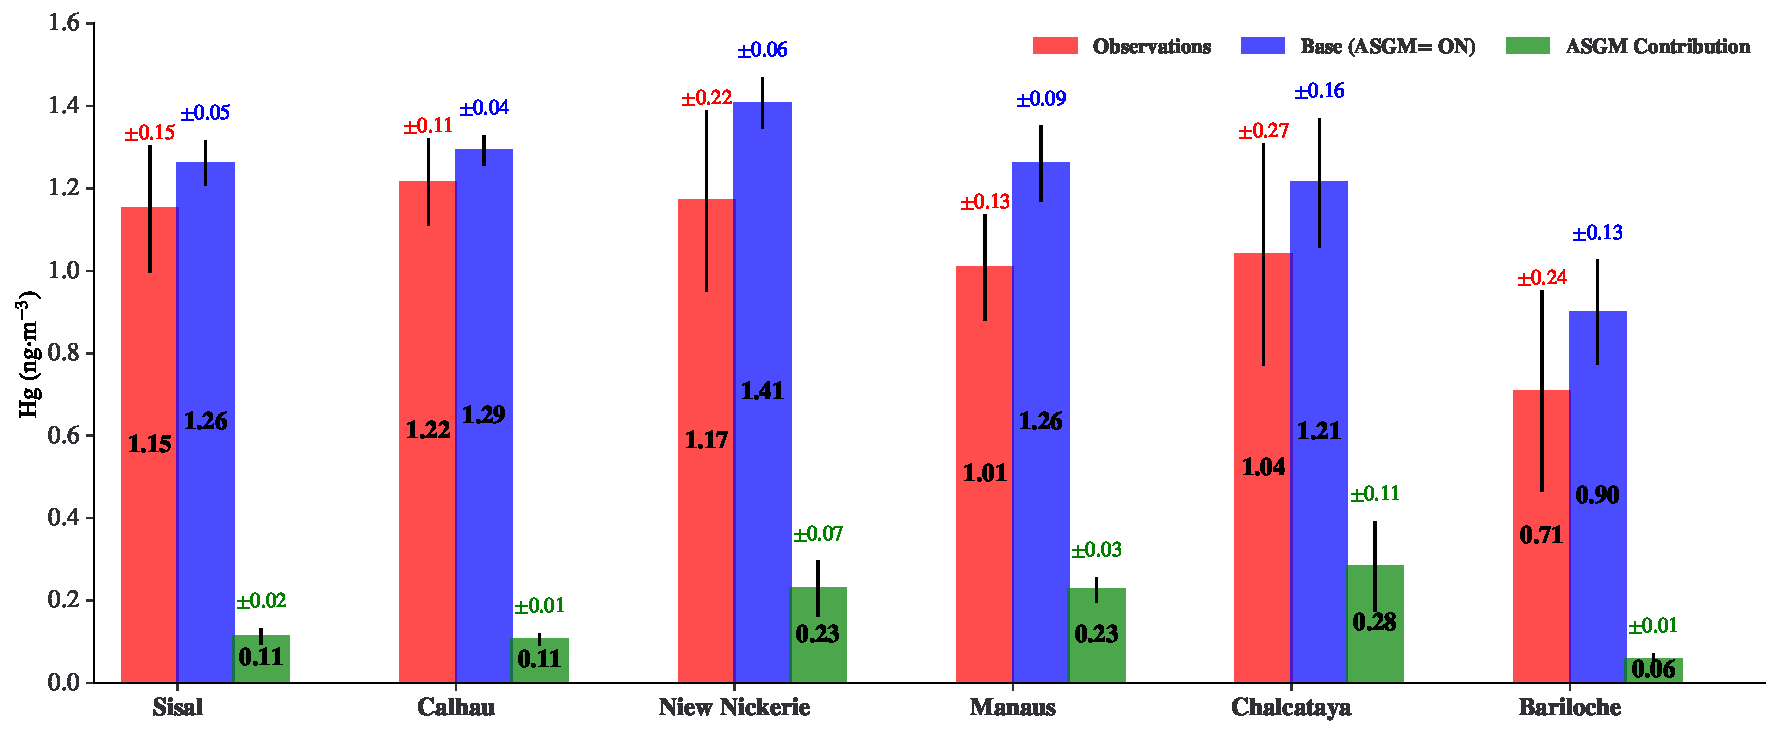
\includegraphics[width=\textwidth]{templates/figures/GMOS_Sites/gmos_sites_stats.pdf}
\centering
\caption[Bar chart comparing the modeled and observed average Hg concentration at the respective GMOS Sites.]{Bar chart comparing the modeled and observed average Hg concentration at the respective GMOS Sites. The blue bars indicate the modeled annual average concentration, the red bars indicate the observed annual average concentration, and the green bars indicate the ASGM contribution at each site. The bars are annotated with the average Hg concentration values. Moreover, the error bars and the annotated value above the bars show the standard deviation in each data set. }
\label{fig:gmos_sites_stats}
\end{figure}
\FloatBarrier

\begin{flushleft}
Figure \ref{fig:gmos_sites_stats} shows that ASGMs modeled contribution is low in most sites except for Chacaltaya, Manaus, and Nieuw Nickerie. The model's behavior regarding the predicted ASGM contribution at these sites is not surprising since these three sites are in countries estimated to be among the top 10 Latin American ASGM Hg emitters in the ASGM emission inventory used for \gc simulation. Even though the model estimates a notable ASGM contribution at the Manaus (18\%) and Nieuw Nickerie (16\%) sites, the sites lack enough data to fully characterize the ASGM contribution to the modeled \hg concentration over the long term. However, the predicted  ASGM Hg contribution at Chacaltaya is the highest at 23\% as seen in Table \ref{tab:model_percentage_overestimation_of_mean}. 
\end{flushleft}

\begin{flushleft}
 As far as the PAS observed GEM concentrations are concerned, the modeled background \hg concentrations in Figure \ref{fig:06-12-22_pas_vs_model_Hg0-per-year_001} seem to match the PAS GEM measurement at Chalcataya, but, according to Quant et al.\cite{quant_measuring_2021}, the higher GEM levels observed at Chacaltaya (1.4\nang) are likely to reflect a known Hg spill near the sampling site and may not reflect regional Hg concentration values. The Chacaltaya Hg spill occurred after the GMOS Chacaltaya site had completed its data collection period. Thus, the GMOS Chacaltaya station's annual average Hg concentration reflects regional Hg concentration more than the PAS station. In comparison with PAS data, the GEOS-Chem model also overestimated atmospheric concentrations. This phenomenon is more prevalent in inland sites than coastal ones. 
 
 \end{flushleft}

\begin{flushleft}
 In the Amazon region, for example, there is a difference between the model and inland PAS sites. This may be because the GEOS-Chem model version used in this study underestimates Hg uptake by plants \cite{feinberg_evaluating_2022}, which means that the model predicts a higher Hg concentration in the atmosphere than it is. Figure \ref{fig:06-12-22_pas_vs_model_Hg0-per-year_by-latitude_001} which shows the modeled (blue circles) and observed (red circles) annual average \hg plotted as a function of latitude indicates the interhemispheric gradient observed in GEOS-Chem. The observation error bars represent the replicate precision of the observations, while the model error bars represent the \nft bootstrap confidence interval for the mean annual \hg. 
\end{flushleft}
 
\begin{figure}[H]
  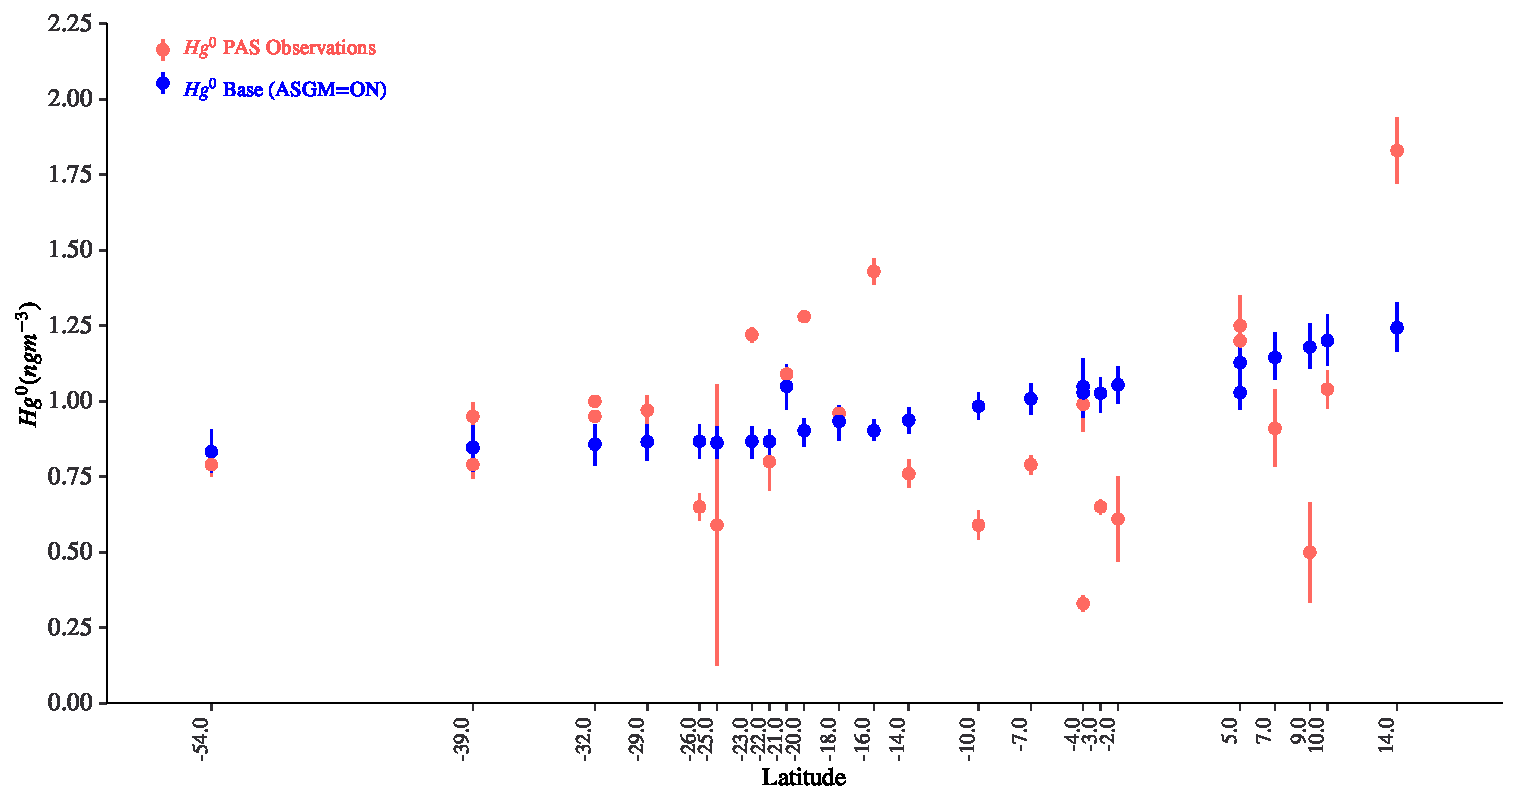
\includegraphics[width=\textwidth]{templates/figures/Passive_Samplers/06-12-22_pas_vs_model_Hg0-per-year_by-latitude_001.pdf}
  \centering
  \caption[Hg Concentration in the atmosphere as a function of Latitude.]{Hg Concentration in the atmosphere as a function of Latitude. The \on (blue circles) and observed (red circles) annual average \hg plotted are plotted as a function of latitude to evaluate spatial trends across the continent. The observation error bars represent the replicate precision of the observations while the model error bars represent the 95\textsuperscript{th} bootstrap confidence interval for the mean annual \hg.}
  \label{fig:06-12-22_pas_vs_model_Hg0-per-year_by-latitude_001}
  
  
\end{figure}
\FloatBarrier
\begin{flushleft}
    \gcs overestimation of Hg concentration in the Amazon region observed above was also addressed in Feinberg et al.\cite{feinberg_evaluating_2022}  where \gc simulations were compared with litterfall, throughfall, and flux tower measurements from 93 forested sites to evaluate vegetation as a Hg sink. The study concluded that the \gc version, 12.8.1 underestimates \hg dry deposition, which may explain why measurements of Hg concentration in Latin America were lower than predicted by \gc. 

\end{flushleft}


\subsection{Modeled vs. Observed Temporal Trends}\label{c2_modeled_vs_observed_trends}
\begin{figure}[H]
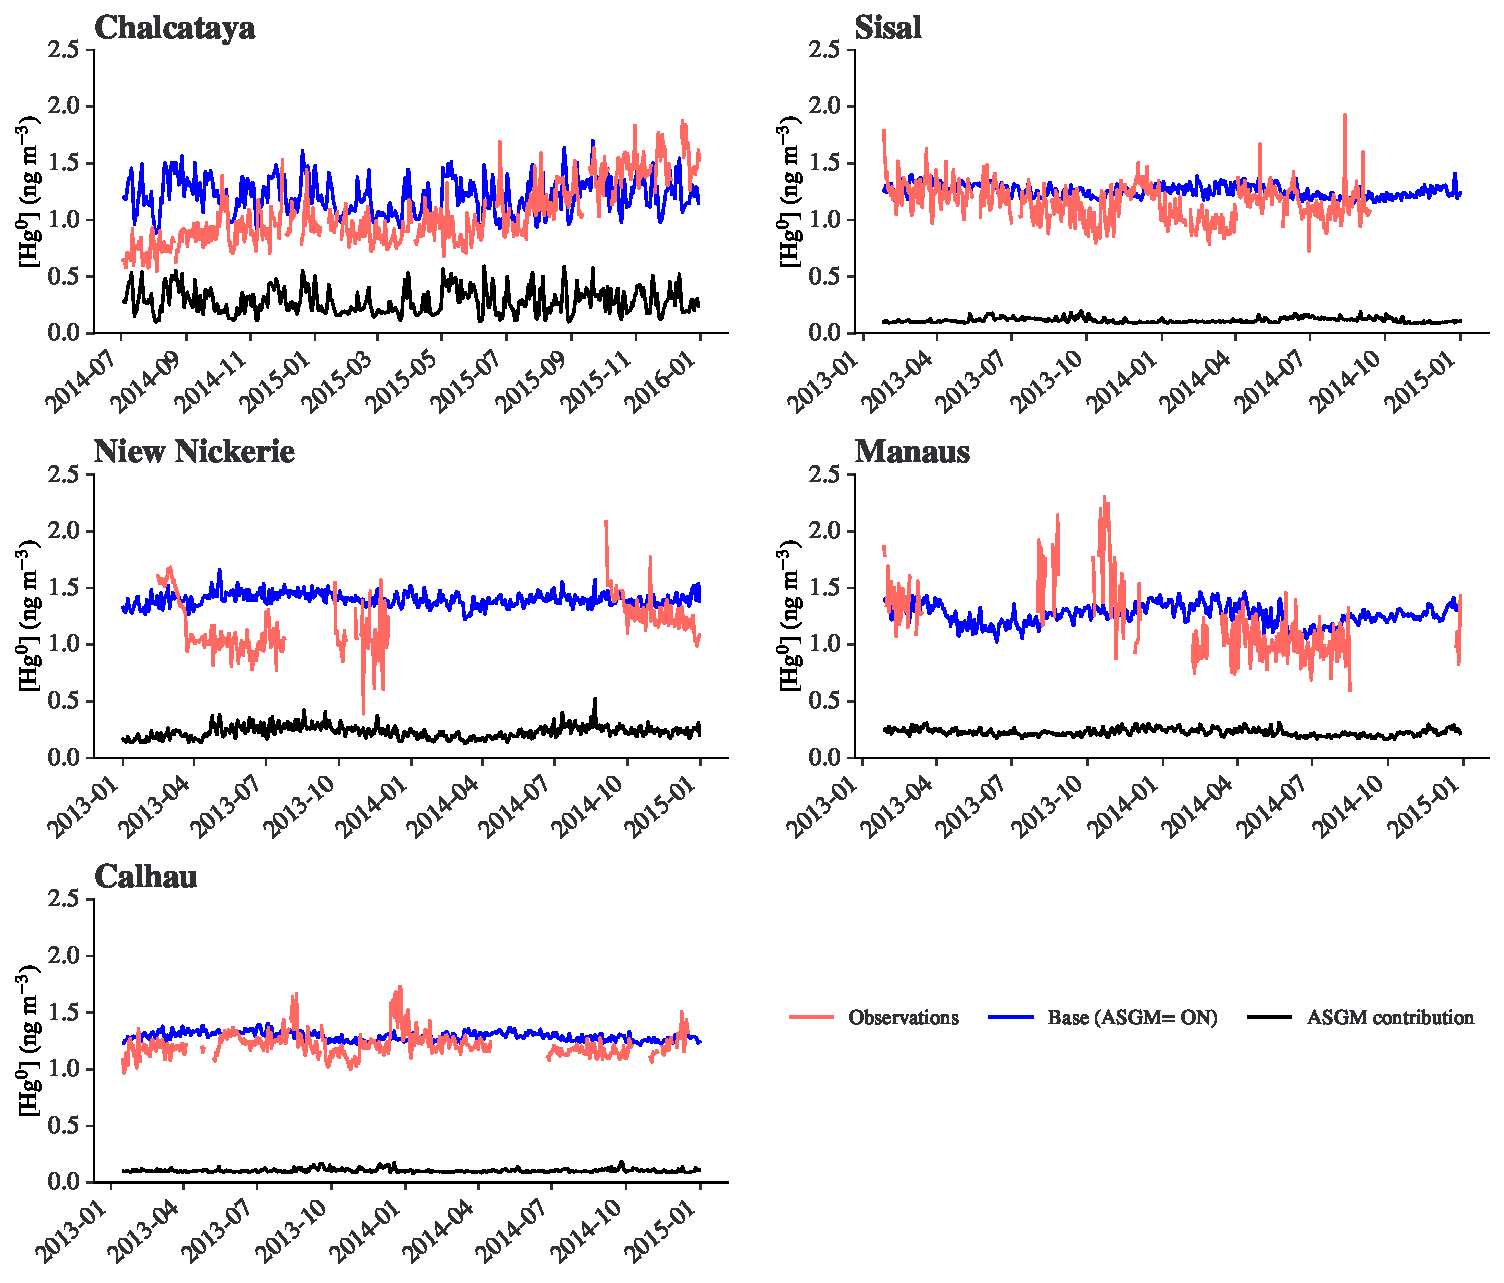
\includegraphics[width=\textwidth]{templates/figures/GMOS_Sites/GMOS_Sites.pdf}
\centering
\caption[Time series plots of the observed TGM concentrations at different GMOS sites.]{Time series plots of the observed TGM concentrations at different GMOS sites in red with the corresponding modeled concentration in blue and the associated ASGM contribution in green. Except for the CHC site, where the data are from July 2014 and January 2016, the available data and corresponding model outputs were plotted between January 2013 and January 2016.}
\label{fig:GMOSvsGC}
\end{figure}
\FloatBarrier


\begin{flushleft}


 This study also compared observed and modeled data on a daily resolution as seen in Figure \ref{fig:GMOSvsGC}, which shows the time series of the modeled \hgc in the atmosphere alongside the observed Hg and the simulated ASGM contribution to the atmospheric Hg concentration at the GMOS sites. The \gc model version used in this study overestimated the concentration of Hg on most days. However, the \gc estimated average \hgc over the available observation period was within one standard deviation of the observed Hg in most of the sites except for the Manaus and Nieuw Nickerie sites. \gcs overestimates the observed GEM concentrations at the Manaus and Bariloche master sites by over 25\%  and the GEM concentration at Nieuw Nickerie by 20\%, which may be indicative of poor parameterization of GEM in the model. Moreover, the overestimation of GEM concentrations in Manaus further indicates the model's poor implementation of Hg plant uptake through dry deposition, as discussed in Feinberg et al.\cite{feinberg_evaluating_2022}.
\end{flushleft}

\begin{flushleft}
 Figure \ref{fig:gmos_sites_scatter} displays the scatter plots of modeled Hg concentrations as a function of the observed Hg concentrations for each site. Each plot uses the red line to evaluate the linear relationship between the modeled and observed Hg concentrations. Equations of the red regression line and the coefficient of determination for each site are also displayed on the plots. The general observation is that the model poorly matched the observations, indicated by the  mild and even flat slopes and shallow $R^2$ values. The low correlations between the model and observations may be attributed to poor vegetation uptake\cite{feinberg_evaluating_2022}. Another plausible hypothesis about the poor model prediction is that the input ASGM emissions that GEOS-Chem uses are poorly parameterized. Wrong emissions in the model may reduce the extent to which the model recreates the observed atmospheric Hg concentrations. Chapter \ref{Chapter3} investigates this hypothesis in detail and highlights some causes, such as the underestimation of emissions from high Hg-emitting regions like Madre de Dios.
 \end{flushleft}


 \begin{figure}[H]
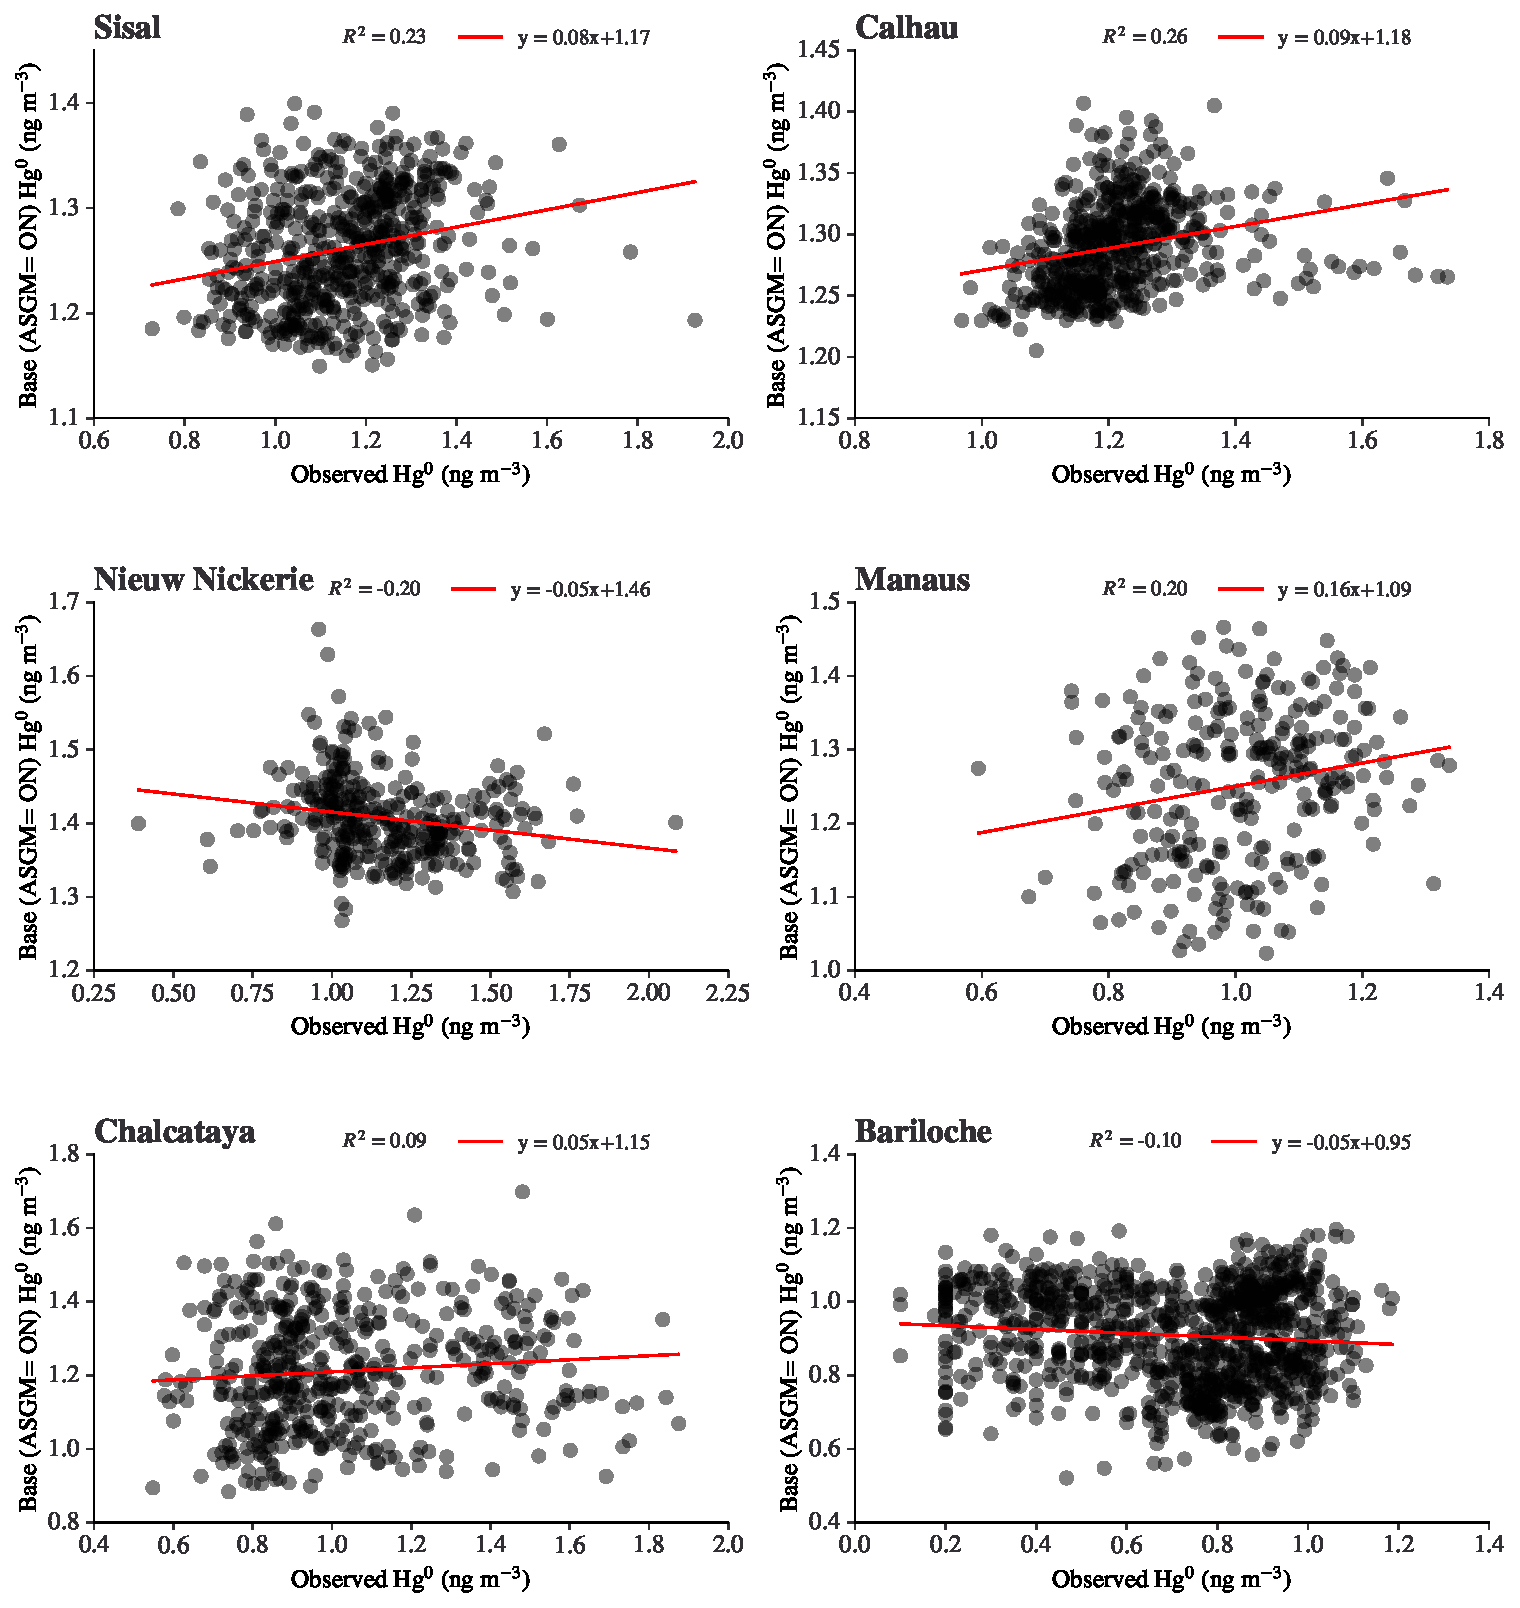
\includegraphics[width=\textwidth]{templates/figures/GMOS_Sites/gmos_sites_scatter.pdf}
\centering
\caption[Scatter plots of the modeled Hg concentration as a function of the observed concentration.]{Scatter plots of the modeled Hg concentration as a function of the observed concentration. The red line is used to investigate the extent of the linear relationship between the modeled and observed Hg concentrations. The coefficient of determination($R^2$) and the equation of the red regression line are shown above each site scatter plot}
\label{fig:gmos_sites_scatter}
\end{figure}
\FloatBarrier

\subsection{Comparison of Model Predictions}
\begin{flushleft}
GEOS-Chem's skill in reproducing the Hg concentration measured using the two sampling methods was analyzed using the scatter plots in Figure \ref{fig:pas_vs_gmos}.  Figure \ref{fig:pas_vs_gmos} (a) shows the modeled annual mean \hgc for each GMOS site as a function of the observed \hgc at the site, while Figure \ref{fig:pas_vs_gmos} (b) shows the modeled annual mean \hgc for each of 6 PAS sites that are the closest to the 6 GMOS sites in (a) as a function of the observed \hgc at the respective site. In each plot, the red line is the regression line to investigate the strength of the association between the modeled concentrations and observed concentrations. 
\begin{figure}[H]
\centering

\begin{tabular}[H]{cc}

\subfloat[GMOS]{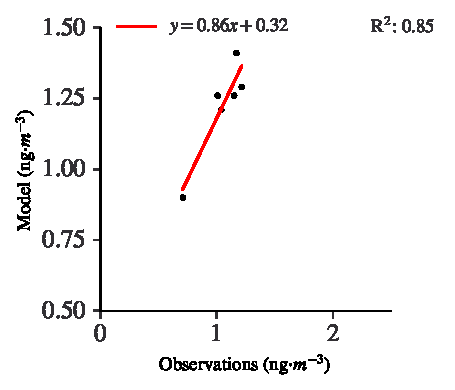
\includegraphics[width = 0.5\linewidth]{templates/figures/07-20-22_gmos-mod_mean_scatter.pdf}}
\subfloat[PAS]{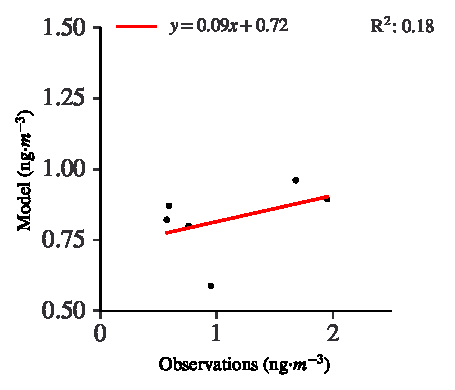
\includegraphics[width = 0.5\linewidth]{templates/figures/07-20-22_pas-mod_mean_scatter.pdf}}


\end{tabular}
  

\captionof{figure}[Scatter plots comparing model's predicted Hg Concentration means with the GMOS and PAS average annual Hg Concentration means]{Scatter plots comparing model's predicted Hg Concentration means with the GMOS and PAS average annual Hg Concentration means. (a) shows modeled annual mean \hgc for each site as a function of the observed \hgc at the site. The red line is the regression line}
\label{fig:pas_vs_gmos}
\end{figure}
\FloatBarrier
Figure \ref{fig:pas_vs_gmos} shows that GEOS-Chem is better at reproducing  the actively monitored average Hg concentration (steep slope and large $R^2$) than the data from the passive monitoring. Furthermore, adding all the remaining Hg concentrations from the PAS did not improve the slope or $R^2$ but worsened the relationship. Even though Figure \ref{fig:gmos_sites_scatter} informs us that GEOS-Chem poorly predicted daily averages at the individual GMOS sites, Figure \ref{fig:pas_vs_gmos} shows that its predictions of actively monitored Hg concentrations are better in aggregate than passively monitored Hg concentrations. This result suggests that modeling studies would gain better insights from comparisons with actively monitored Hg concentrations. However, this result does not render PAS monitoring obsolete. Using PAS technologies, we can obtain high-quality data about Hg concentrations in the atmosphere and understand regional background Hg concentrations over long periods. Since PAS networks are relatively inexpensive and easy to install, countries can use them to understand their Hg emissions better, providing valuable global and regional monitoring data. A better understanding of temporal trends can be gained from active monitoring, as evidenced by the analysis of GMOS TGM concentrations.
Furthermore, a single data set of actively monitored Hg concentrations can be analyzed to generate metrics such as mean, \iq, and \nft, allowing multiple ways to compare modeled and observed concentrations. Despite  not recreating the exact Hg concentrations  observed at GMOS sites, improvements to the model, such as the update in the model's dry deposition discussed in Feinberg et al.\cite{feinberg_evaluating_2022} may improve the \gcs predictions of measured Hg concentration in the atmosphere. Additionally, Shah et al.'s\cite{shah_improved_2021} improved mechanistic model of the atmospheric redox chemistry of mercury may also reduce  GEOS-Chems's error in predicting the observed concentrations.
\end{flushleft}

\section{Conclusion}\label{c2_conclusion}
\begin{flushleft}
This chapter explored the relationship between the modeled and observed Hg concentrations in Latin America. The atmospheric Hg measurements from six active monitoring sites  across Latin America part of the GMOS network were analyzed and compared with modeled \hg concentrations at the respective sites\cite{koenig_seasonal_2021,sprovieri_atmospheric_2016}. Furthermore, annual average GEM measurements from 27 PAS sites across Latin America were compared to 1-year beverages for \hg concentrations at the respective monitoring sites \cite{quant_measuring_2021}.  A relatively weak relationship was found between the observed mercury species (GEM and TGM) and those in the \on, demonstrating a need for improving the models. Additionally, GEOS-Chem recreated the average Hg concentration measurements from active monitoring stations better than PAS. Lastly, improved vegetation uptake and more accurate emission parameterizations may improve the model's prediction.

\end{flushleft}